\documentclass[12pt,a4paper, ngerman, oneside]{scrartcl}
\usepackage[ngerman]{babel}
\usepackage[utf8]{inputenc}
%\usepackage[T1]{fontenc}
%\usepackage{lmodern}
\usepackage{ucs}
\usepackage{amsmath}
\usepackage{amsfonts}
\usepackage{amssymb}
\usepackage{graphics}
\usepackage{paralist}
\usepackage[linkcolor=black]{hyperref}
\usepackage{listings} \lstset{numbers=left, numberstyle=\tiny, numbersep=5pt} \lstset{language=Java}
%% Grafiken
\usepackage[pdftex]{graphicx}
\usepackage{epsfig} 
\hypersetup{% 
  colorlinks=true,
}

\newcommand\blfootnote[1]{%
  \begingroup
  \renewcommand\thefootnote{}\footnote{#1}%
  \addtocounter{footnote}{-1}%
  \endgroup
}

\hypersetup{
  pdfborder = {0 0 0},
  urlbordercolor = {0 0 0},
  colorlinks = true,
  linkcolor = black,
  citecolor = black,
  filecolor = black,
  urlcolor  = black
}
% Variablen
\newcommand{\Tiles}{\emph{8}}
\newcommand{\Rundenlimit}{\emph{20}}
\newcommand{\PointsPerTile}{\emph{7}}
\newcommand{\PointsPerPassenger}{\emph{7}}
\newcommand{\FieldsPerTile}{\emph{20}}
\newcommand{\Passagiere}{\emph{5}}


\sloppy
\hyphenpenalty=100000

\date{Software-Challenge Germany 2017\\Stand \today}


%\author{Niklas Paulsen, npau@informatik.uni-kiel.de }
\title{Spielanleitung Mississippi Queen}


\begin{document}
\maketitle
%\begin{figure}[!htbp]
%  \centering
%  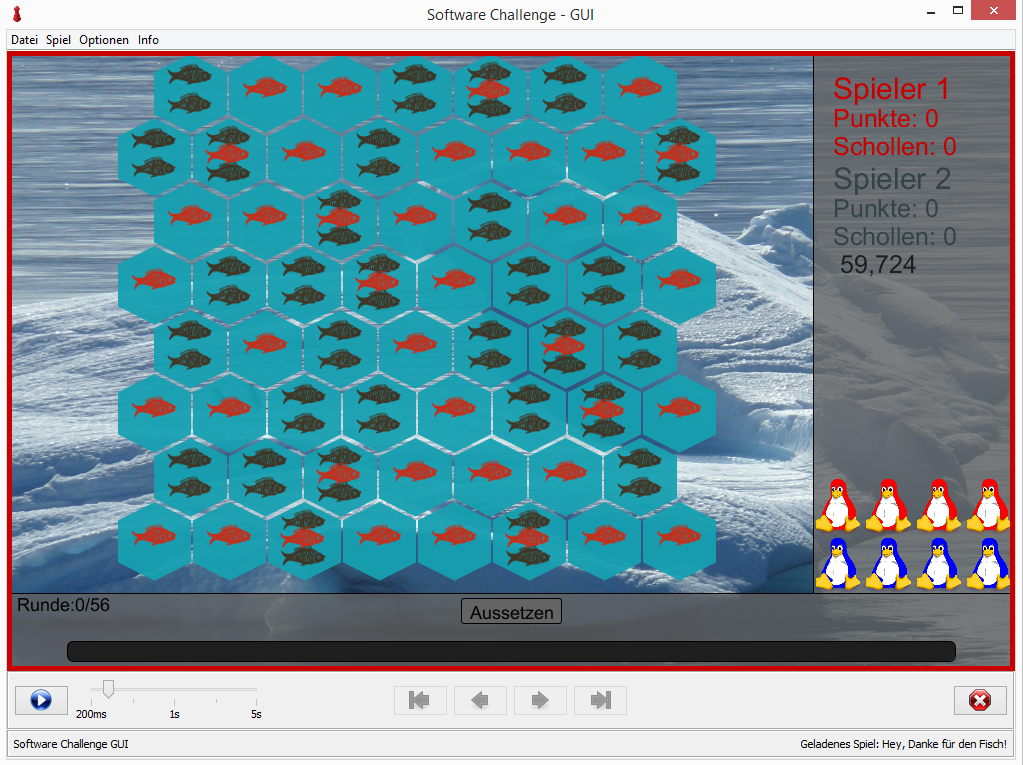
\includegraphics[width=\linewidth]{bilder/gui.png}
%\end{figure}
\vspace*{\fill}

%\blfootnote{Die Nutzung des Spielkonzeptes "`Twixt"' (Name, Spielregeln und Grafik)
%  erfolgt mit freundlicher Genehmigung des Kosmos Verlags.}

\newpage
\tableofcontents
\thispagestyle{empty}
\newpage
\setcounter{page}{1}
\section{Einleitung}
In dieser Anleitung werden die Elemente und Regeln des Spiels Mississippi Queen der
Software-Challenge 2017 erläutert.
Bei Mississippi Queen versuchen zwei Spieler, durch abwechselndes setzen von Raddampfern 
schnellstmöglich einen Fluss bis zum Ziel entlangzufahren und dabei zwei Passagiere mitzunehmen.
Der Spieler, der zuerst im Ziel gewinnt das Spiel.
\section{Das Spielbrett}
Ein Ausschnitt des Spielbretts ist im Titelbild zu sehen. Es besteht aus \emph{\Tiles} Spielsegmenten. Mit jeweils \emph{\FieldsPerTile} Feldern. Am Anfang ist das Startsegment und ein darauffolgendes Segment aufgedeckt. Sobald ein Spieler das letzte Segment betritt, wird ein neues dahinter zufällig links, rechts oder mittig angebaut. Dies geschieht solange, bis keine Segmente mehr übrig sind. Das letzte Segment ist das Zielsegment (TODO Graphik einfügen darin Zielfelder markieren). Segmente die schon von allen Spielern betreten wurden, werden vom Spielplan entfernt, auch wenn sich darauf noch Passagiere befinden. Es sind anfangs nur die ersten beiden Spielsegmente aufgedeckt. Sobald ein Spieler das letzte sichtbare Segment betritt, wird ein neues hinzugefügt.
Die Inselfelder sind dabei zufällig auf der Karte verteilt. Insgesamt gibt es \emph{\Passagiere} Passagierfelder. Sandbänke und Baumstämme werden ebenfalls zufällig eingefügt.
\subsection{Das Wasserfeld (WATER)}
Das Wasserfeld (WATER) kann ganz normal befahren werden. Auf ein zum Spieler benachbarten Wasserfeld ziehen kostet einen Geschwindigkeitspunkt.
\subsection{\label{water}Das Inselfeld (BLOCKED)}
Das Inselfeld (BLOCKED) kann nicht überquert werden.
\subsection{Das Passagierfeld in Richtung i (PASSENGERi)}
Das Passagierfeld mit Anleger in Richtung i enthält einen Passagier, der am entsprechenden Anleger abgeholt werden kann, wenn man das Feld mit Geschwindigkeit 1 erreicht und dann der Zug beendet wird. Es verwandelt sich in ein normales Inselfeld, sollte der Passagier abgeholt werden (siehe \ref{water})
\subsection{Das Zielfeld (GOAL)}
Das Zielfeld ist ein Feld, dass erreicht werden kann, um das Spiel zu gewinnen. Dabei muss die Geschwindigkeit 1 sein und 2 Passagiere müssen eingeladen worden sein.
\subsection{Die Sandbank (SANDBAR)}
Eine Sandbank bringt ein Schiff in der Bewegung zum halten, sollte man darauf fahren. Es kann nur rückwärts oder vorwärts dann aber unter Verwendung von einer Kohleeinheit verlassen werden. Auf einer Sandbank kann nicht gedreht werden und ein Spieler der sich darauf befindet kann nicht abgedrängt werden. Das Fahren auf eine Sandbank beendet den Zug und setzt die Geschwindigkeit des Schiffes auf 1.
\subsection{Das Baumstammfeld (LOG)}
Ein Baumstammfeld ist ein Feld, dass die doppelte Anzahl an Bewegungspunkten braucht, um es zu überqueren.
Außerdem wird die Geschwindigkeit eines Schiffes, welches ein Baumstammfeld durchquert nach dem Zug um 1 verringert. Sind nicht genug Bewegungspunkte vorhanden, kann es nicht überquert werden. Das Abdrängen in ein Baumstammfeld kostet einen zusätzlichen Bewegungspunkt.TODO Bilder mit Feldern einfügen

\section{Spielablauf}
Beide Spieler starten mit Geschwindigkeit 1 und 6 Kohleeinheiten und ziehen dann abwechselnd. Ein Zug besteht aus mehreren Aktionen. In allen Aktionen müssen (falls der Zug nicht auf einer Sandbank endet) insgesamt alle Bewegungspunkte (bestimmt durch die Geschwindigkeit des Schiffes) verbraucht werden. In den folgenden Kapiteln werden diese beschrieben:
\subsection{\label{acceleration}Beschleunigungsaktion}
Kann nur als erste Aktion ausgeführt werden. Die Beschleunigung um eine Geschwindigkeitseinheit ist frei, jede Beschleunigung um mehr als 1, kostet für jeden weiteren Geschwindigkeitspunkt eine Kohleeinheit. Die Höchstgeschwindigkeit ist 6, die niedrigste ist 1. Eine Beschleunigungsaktion um 0 ist ungültig.
\subsection{\label{turn}Drehaktion}
Eine Drehaktion im Zug des Spielers eine Einheit ist frei (Ausnahme \ref{push}). Jede weitere Drehung erfordert eine Kohleeinheit. Es kann sich nicht auf Sandbänken gedreht werden. 
\subsection{\label{push}Abdrängaktion}
Zieht ein Spieler auf ein Feld, auf dem sich der gegnerische Spieler befindet, muss darauf eine Abdrängaktion folgen. Ein Spieler kann den Gegner auf ein beliebiges, angrenzendes, nicht direkt hinter den Spieler liegendes, begehbares Feld abdrängen (\label{passierbar}Wasserfelder, Sändbänke und Baumstammfelder gelten als begehbar). Eine Abdrängaktion kostet einen Bewegungspunkt, zwei, falls auf ein Baumstammfeld abgedrängt wird. Es darf nicht von einer Sandbank aus abgedrängt werden. Der abgedrängte Spieler bekommt (außer er wurde auf eine Sandbank abgedrängt, wobei sich auch in diesem Fall seine Geschwindigkeit auf eins reduziert) eine zusätzliche freie Drehung für seinen nächsten Zug.
\subsection{\label{step}Bewegungsaktion}
Eine Bewegungsaktion erfolgt in die derzeitige Richtung des Schiffes des Spielers. Sie kann nur über und auf passierbare (siehe \ref{passierbar} Felder erfolgen. Sie darf auf dem Feld des Gegners oder eine Sandbank enden, aber niemals durch ein vom Gegner besetztes Feld oder eine Sandbank gehen.  
\section{Spielende}
Das Spiel endet, sobald ein Spieler mit 2 Passagieren ein Zielfeld erreicht hat, sobald das Rundenlimit von \emph{\Rundenlimit} Runden erreicht ist oder falls nach dem Zug des Spielers der nicht Startspieler war ein Spieler vier oder mehr Spielsegmente zurückliegt. Wird das Rundenlimit erreicht gewinnt der Spieler mit den meisten Punkten. Die Punkte errechnen sich folgendermaßen:
\begin{itemize}
\item Jeder eingesammelte Passagier bringt 5 Punkte
\item Jedes überwundene Segment bringt 5 Punkte. 
\item Anhang der Position innerhalb eines Segments werden 0 bis 4 Punkte vergeben. (Ein Segment ist aufgeteilt in 5 Reihen je weiter vorne man ist, desto mehr Punkte bekommt man TODO siehe Graphik).
\end{itemize}
Der Spieler mit den meisten Punkten gewinnt dann das Spiel. Sollten beide Spieler gleich viele Punkte haben, gewinnt der Spieler, der mehr Passagiere eingesammelt hat. Sollte auch diese Zahl gleich sein, endet das Spiel unentschieden.
\section{Graphische Benutzeroberfläche}
TODO

\end{document}
